%
\subsection{Remote Client}
\label{sec:remote-cli-decomp}
%
In this section the remote client is analyzed, considering its events, use cases, dynamic operation and the flow of events.

\subsubsection{User mockups}
\label{sec:user-mockups-1}
%
In Fig.~\ref{fig:user-mockups-rc} is illustrated the user mockups for the remote client. 
It intends to clarify how does the~\gls{ui} works for the two different sides: Brands and Company (staff).

The initial state of the~\gls{mdo-rc}'s~\gls{ui} is depicted in thick border outline: the 'Sign In' window. 
If the \texttt{User} makes a mistake in its username and/or password, it will be shown an error message. 
Also, the 'Sign In' window has an option to recover the password, which sends an e-mail to switch password.
If the \texttt{User} still remembers its credentials, the app flows through one out of two possibilities: if the user is an admin, goes to the admin main menu, or else if the user is a brand, it will appear the brand main menu.

Firstly, the \texttt{Admin} workflow:
%
\begin{itemize}
\item The \texttt{Admin} main menu contains a drop down button with all the stations available. Choosing one of them, the \texttt{Admin} can turn it On/Off, see it's current mode and the current brand ad being displayed. Also, the \texttt{Admin}  can log out and choose between two different paths:
%
\begin{itemize}
\item \emph{Statistics}: It is possible to see various statistics of all different brands that are currently playing on the station: the number of times that the ad was shown, the number of pictures/\gls{gif}s and shared posts, the fragrance slot and quantity (percentage) and the days remaining for the rent to end.
It is also possible to deactivate the add if something wrong occurs and go back to the previous menu.
\item \emph{Users}: In this window, the admin can manage all users and see their information.
It is possible to the admin to change the type of user to brand or to admin, and it can also remove its type.
Also, the admin can delete users from the database. 
\item \emph{Ads to Activate}: In this window, the \texttt{Admin} can handle all the ads that the brands are intending to rent.
For that, the \texttt{Admin} needs to see if everything is in order, such as if all the videos that the brand wants to display are in order (in case there are some  or decontextualized videos), if it has a filter, a fragrance and a slot.
After that, the \texttt{Admin} can either accept or deny the ad.
If it accepts the ad, it is shown a success message and the ad is added to the station with its preferences.
If the ad is denied, the \texttt{Admin} needs to send a reason why it denied the ad, that is consequently send to the brand's email.
\end{itemize}
%
\end{itemize}

Secondly, the \texttt{Brand} workflow:
\begin{itemize}
\item The \texttt{Brand} main menu contains a welcome message, a notification bell to see if another ad was accepted or denied and three buttons - Rented, To Rent and Log Out.
The 'Log Out' button logs the \texttt{Brand} out of its account, the other two buttons switch to different widgets:
%
\begin{itemize}
\item \emph{Rented}: The \texttt{Brand} can see all statistics of all its rented ads on different stations that it rented.
That statistics are: status, number of times the ad was shown, the fragrance slot and quantity (percentage), the number of pictures/\gls{gif}s taken, the number of shared posts and the number of days remaining to end its rent.
The 'Go Back' button goes back to the previous menu.
\item \emph{To Rent}: The \texttt{Brand} can rent ads in the same station or in other stations.
To that happens, it is only needed to choose the target hours and then a calendar will show what days are available to that hours, then after choosing the days, the \texttt{Brand} need to upload a filter and a .zip file with a maximum of ten videos. 
Finally, the \texttt{Brand} needs to select the fragrance that wants to spill to the air and select 'Rent'. After that, a success message will be shown and the ad will enter in wait list for an \texttt{Admin} check if everything is in order.
\end{itemize}
%
\end{itemize}

It is also possible to register a new user through the 'Register' button.
This opens a window to type a username, a password, confirm the password and the e-mail.
If everything is in order, the user is created with the default user type of Brand.

Finally, at any time, it can occur the loss of internet connection, which toggles an error message informing the automatic log out of the account.
\begin{figure}[htb!]
\centering
    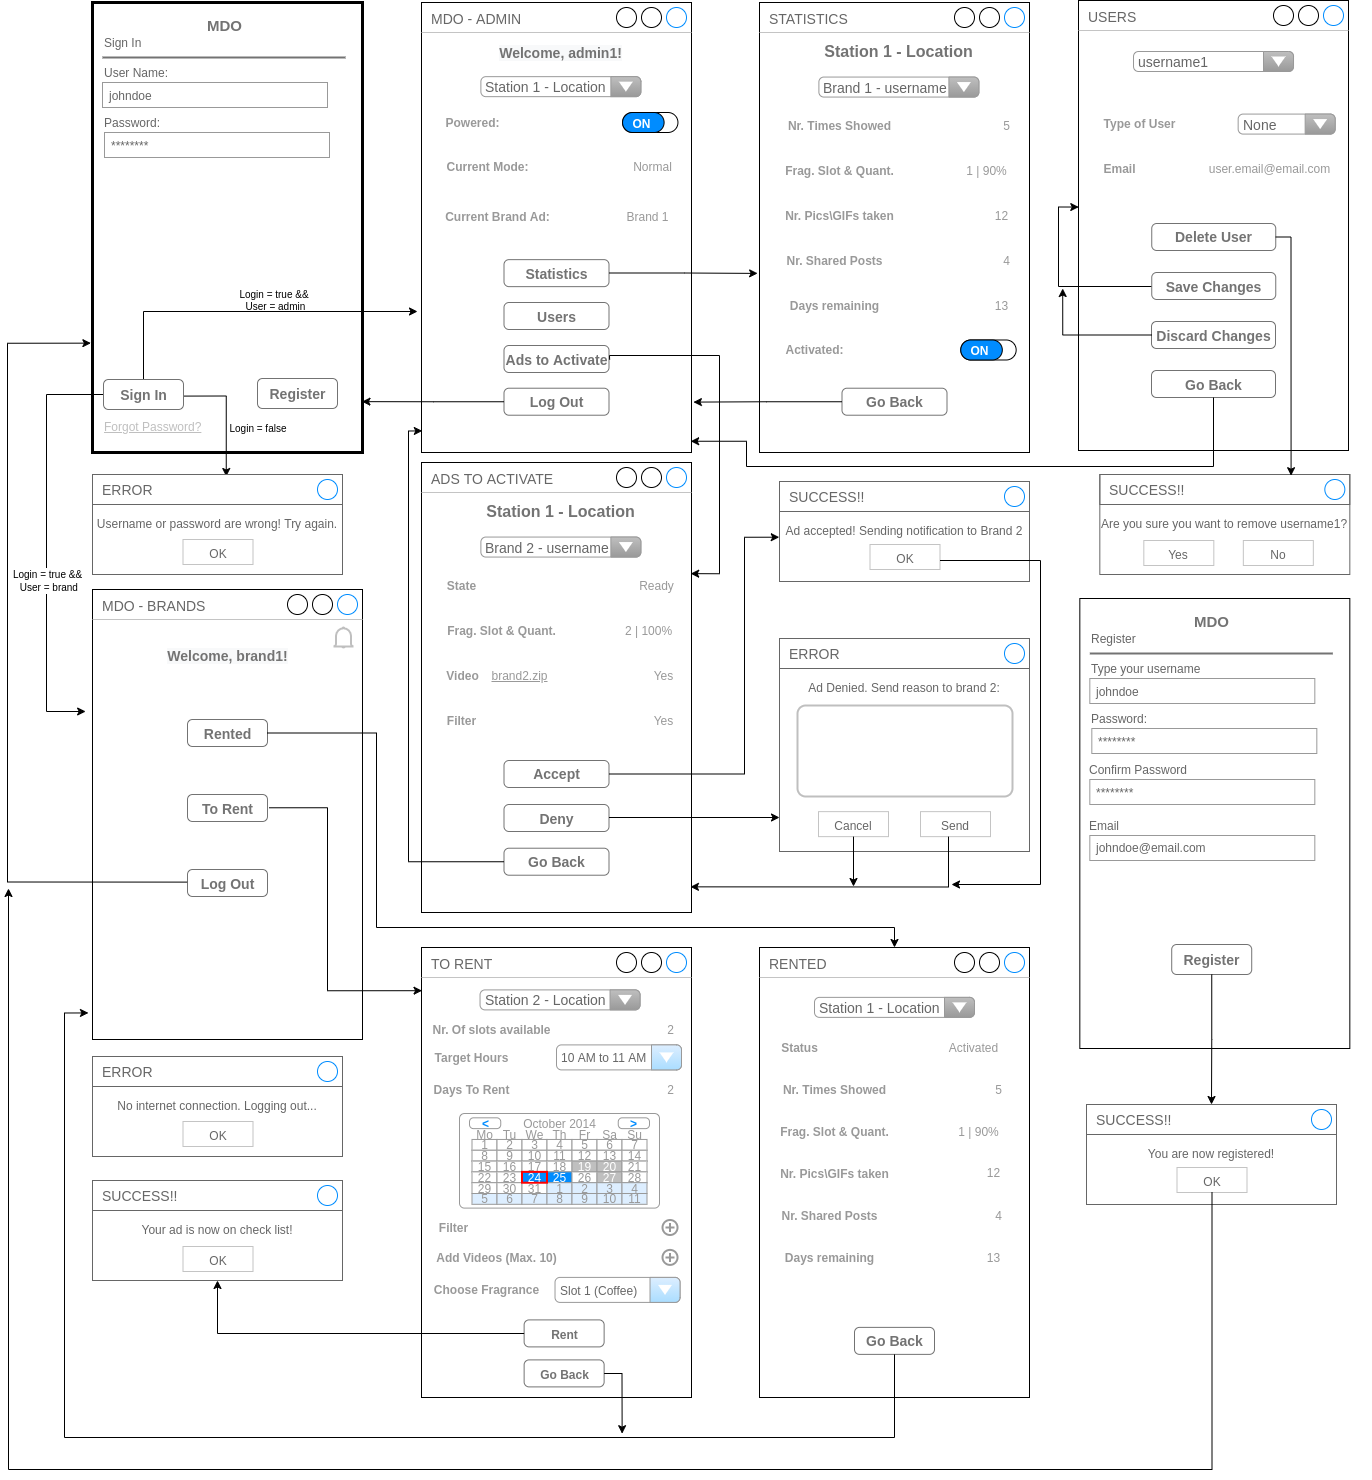
\includegraphics[width=0.9\columnwidth]{./img/user-mockups-rc.png}
  \caption{User mockups: remote client}%
\label{fig:user-mockups-rc}
\end{figure}

\subsubsection{Events}
\label{sec:events-1}
Table~\ref{tab:events-rc} presents the most relevant events for the Local system, categorizing them by their source and
synchronism and linking it to the system’s intended response.

%
\begingroup
\renewcommand{\arraystretch}{0.7} % Default value: 1
% Please add the following required packages to your document preamble:
% \usepackage{graphicx}
\begin{table}[]
\centering
\caption{Events: remote client}
\label{tab:events-rc}
\resizebox{\textwidth}{!}{%
\begin{tabular}{llll}
\hline
\textbf{Event} &
  \textbf{System response} &
  \textbf{Source} &
  \textbf{Type} \\ \hline
Login &
  \begin{tabular}[c]{@{}l@{}}The system verifies if the user credentials\\ are correct and what type of user is and\\ asks for data from databases\end{tabular} &
  User &
  Asynchronous \\ \hline
Verify internet connection &
  Periodically verify internet connection &
  Remote Client &
  Synchronous \\ \hline
Statistics &
  \begin{tabular}[c]{@{}l@{}}Request to the Remote Server all the\\  information to show statistics from \\ all stations and brands\end{tabular} &
  User (Admin) &
  Asynchronous \\ \hline
Accept/Deny ad &
  \begin{tabular}[c]{@{}l@{}}Send information to the Remote \\ Server if the ad is either accepted\\ or denied and if so, why\end{tabular} &
  User (Admin) &
  Asynchronous \\ \hline
Power On/Off Station &
  \begin{tabular}[c]{@{}l@{}}Send command to Remote Server\\  to Power On/Off a certain station\end{tabular} &
  User (Admin) &
  Asynchronous \\ \hline
Rented &
  \begin{tabular}[c]{@{}l@{}}Request to the Remote Server all the\\  information to show statistics from \\ all stations the brand rented\end{tabular} &
  User (Brand) &
  Asynchronous \\ \hline
Rent &
  \begin{tabular}[c]{@{}l@{}}Send to the Remote Server all the \\ information of rent from the brand, \\ all the videos and the filter\end{tabular} &
  User (Brand) &
  Asynchronous \\ \hline
Forgot Password &
  \begin{tabular}[c]{@{}l@{}}Send e-mail to the user that has \\ forgotten his password\end{tabular} &
  User &
  Asynchronous \\ \hline
\end{tabular}%
}
\end{table}
%
%
%
\subsubsection{Use cases}
\label{sec:use-cases-1}
%
Fig.~\ref{fig:use-cases-rc} depicts the use cases diagram for the \texttt{Remote Client}, describing how the system should respond under various conditions to a request from one of the stakeholders to deliver a specific
goal.

The \texttt{Admin} and the \texttt{Brand} interact with the \texttt{Remote Client} and this last interacts with the \texttt{Remote Server} to process commands, such as query databases or power on/off machines.

The \texttt{Admin} can Manage the Station, which includes Power On/Off Station, Manage Ads to Activate and Enable/Disable an Ad.
It can also manage users, removing or modifying them. All these use cases are processed from the \texttt{Remote Client} and are requested to the \texttt{Remote Server}.

The \texttt{Brand} can see Rented Ads, Rent Ads, See notifications and register. All these cases are also processed from the \texttt{Remote Client} and are requested to the \texttt{Remote Server}.

There are some use cases that are common to the  \texttt{Admin} and to the \texttt{Brand}: Login and Logout.


\begin{figure}[htb!]
\centering
    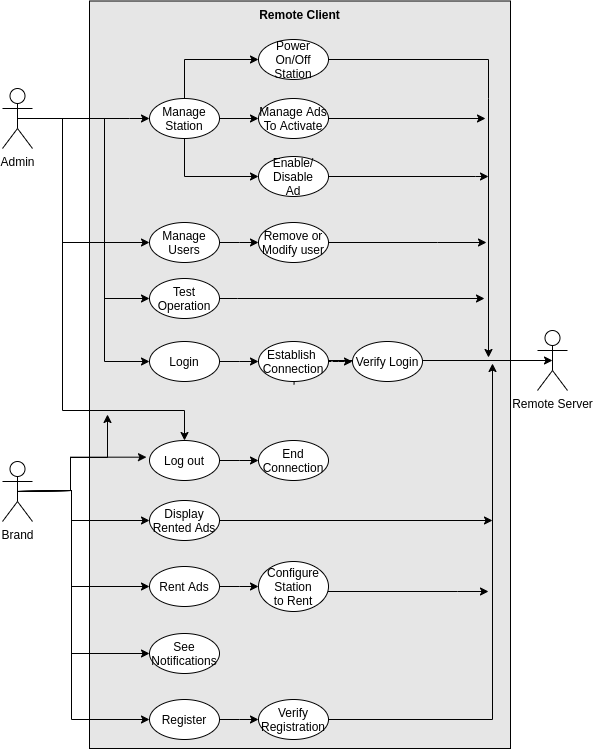
\includegraphics[width=0.9\columnwidth]{./img/use-cases-rc.png}
  \caption{Use cases: remote client}%
\label{fig:user-cases-rc}
\end{figure}


\subsubsection{Dynamic operation}
\label{sec:dyn-oper-1}
State machine diagram

\subsubsection{Flow of events}
\label{sec:flow-events-1}
Sequence diagram

%%% Local Variables:
%%% mode: latex
%%% TeX-master: "../../../dissertation"
%%% End:
